% !TeX spellcheck = de_DE
\documentclass[ngerman]{scrartcl} 

\KOMAoptions{fontsize=12pt, paper=a4}
\KOMAoptions{DIV=11}
\usepackage[utf8]{inputenc}             % Direkte Eingabe von ä usw.
\usepackage[T1]{fontenc}               	% Font Kodierung für die Ausgabe
\usepackage{babel}                   	% Verschiedenste sprach-spezifische Extras
\usepackage{parskip}
\usepackage[autostyle=true]{csquotes}	% Intelligente Anführungszeiche
\usepackage{amsmath}					% Mathematischer Formelsatz mit zusätzlichen mathematischen Schriften und Symbolen
\usepackage{amssymb}					% Mathematischer Formelsatz mit zusätzlichen mathematischen Schriften und Symbolen
\usepackage{physics}					% Differentialgleichungen
\usepackage{listings}					% Zum Einbinden von Programmcode verwenden wir das listings-Paket
\usepackage[dvipsnames]{xcolor}			% um Elemente von Befehlen farblich zu unterstützen
\usepackage[varg]{txfonts}              % Schönere Schriftart
\usepackage{graphicx}					% Paket um externe Graphiken einzufügen
\usepackage{media9}
\RequirePackage[backend=biber, style=numeric]{biblatex} % Literaturverzeichnis
\usepackage{hyperref} 					% um klickbare Elemente in Ihrem PDF-Ausgabedokument zu erzeugen
\RequirePackage[all]{hypcap} 			% ergänzend zu hyperref
\usepackage{siunitx}					% Intelligentes Setzten von Zahlen und Einheiten
\usepackage{enumitem}					% Aufzählungsarten
\usepackage{fancyhdr}


\setlength\parindent{0pt} 				% Sets paragraph indentation to 0

\lstset{									% Deutsche Umlaute
	basicstyle=\ttfamily,    
	literate={~} {$\sim$}{1} 				% set tilde as a literal
	{ö}{{\"o}}1
	{ä}{{\"a}}1
	{ü}{{\"u}}1
	{ß}{{\ss}}1
	{Ö}{{\"O}}1
	{Ä}{{\"A}}1
	{Ü}{{\"U}}1
}

\lstset{
	numbers=left, 						% Line numbering
	numberstyle=\footnotesize, 			% Size of numbers
	basicstyle=\ttfamily\small, 		% Style and Size of Text
	backgroundcolor=\color{White}, 		% Background Color
	language=Python, 					% Language of Code
	commentstyle=\color{Maroon}, 		% Color and Style of Comments
	stringstyle=\color{OliveGreen}, 	% Color of Strings
	showstringspaces=false,
	morekeywords={import,from,class,def,for,while,if,is,in,elif,else,not,and,or,print,break,continue,return,True,False,None,access,as,del,except,exec,finally,global,import,lambda,pass,print,raise,try,assert}, 									% Definition of new keywords that will be highlighted
	keywordstyle=\color{RoyalBlue}		% Color and Style of Keywords
}


\pagestyle{fancy}
\fancyhf{}
\rhead{Ben Karcher, Anika Hoverath}
\lhead{Computerphysik - Abgabe 5}
\rfoot{Seite \thepage}

\title{Computerphysik - Abgabe 5}
\date{\today}


\begin{document}
	% Auf 3 setzen, da es beim ersten Chapter um 1 hochgezählt wird. 3+1=42
	\setcounter{section}{9}
	\thispagestyle{fancy}
	\renewcommand{\thesection}{H.\arabic{section}:}
	\renewcommand{\thesubsection}{H\arabic{section}.\arabic{subsection}}
	
\section{Solitonlösungen der \textsc{Korteweg-de Vries}-Gleichung}

\textit{In diesem pdf-Dokument sind Videos eingebunden, diese werden von \emph{okular} angezeigt. Sollte Ihnen diese nicht angezeigt werden, haben wir die .mp4-Dateien auch nochmal separat angefügt.}

In dieser Aufgabe untersuchen wir Lösungen der Korteweg-de Vries-Gleichung.
Diese Gleichung beschreibt die Ausbreitung von Wellen in Kanälen.

\begin{equation*}
\frac{\partial}{\partial t} u(t, x)=6 u(t, x) \frac{\partial}{\partial x} u(t, x)-\frac{\partial^{3}}{\partial x^{3}} u(t, x)
\end{equation*}

Ein besonderer Satz Lösungen sind die Solitonen.
Diese beschreiben einzelne Wellen, die sich mit konstanter Geschwindigkeit bewegen, ohne zu zerfließen.
Die Anfangsbedingung:

\begin{align}
	u^{[N]}(0,x)=\frac{-N(N+1)}{cosh^2(x)}
\end{align}

erzeugt N Solitonen, die sich mit verschiedenen Geschwindigkeiten ausbreiten.
\subsection{}

Zunächst betrachten wir die analytische Lösung zu $u^{[2]}$:
\begin{equation*}
u^{[2]}(t, x)=-12 \frac{3+4 \cosh (2 x-8 t)+\cosh (4 x-64 t)}{\{3 \cosh (x-28 t)+\cosh (3 x-36 t)\}^{2}}
\end{equation*}

im Bereich $t\in[-1,1]$. 
In Video \ref{vid:H10.1} sieht man, dass zwei Solitonen erzeugt werden.
Um die Geschwindigkeit der Solitonen zu bestimmen, kann man die Position bei $t=1$ ablesen,
da beide Solitonen zur Zeit $t=0$ am Ort $x=0$ anfingen. Dabei ergibt sich:
\begin{align*}
	v_1&=3.45\\
	v_2&=16.27
\end{align*}
\begin{figure}[htbp]
	\centering
	\includemedia[
	width=0.5525\linewidth,height=0.5\linewidth,
	activate=pageopen,
	transparent,
	addresource=Exact.mp4,
	flashvars={
		source=Exact.mp4     % same path as in addresource!
		&loop=true           % loop video
		&scaleMode=letterbox % preserve aspect ratio
	}
	]{}{VPlayer9.swf}
	\caption[2 Solitonen]{Darstellung von $u^{[2]}(x)$ im Bereich von $t\in[-1,1]$}
	\label{vid:H10.1}
\end{figure}
\subsection{}
Nun lösen wir $u^{[N]}$ numerisch.
Dazu nutzen wir die Zeitdiskretisierung $t_n = n \cdot d$ mit der Zeitschrittweite $d$
und die Ortsdiskretisierung $h_j = j \cdot h$ mit der Schrittweite $h$.
Mit der Notation: $u_j^n=u(t_n,x_j)$ lassen sich die einzelnen Teile der partiellen Differentialgleichung schreiben als:
\begin{align*}
	\frac{\partial}{\partial t}u(t,x) \bigg|_{t=t_n, x=x_j} &=\frac{u_j^{n+1}-n_j^{n-1}}{2d} + \mathcal O(d^2) \\
	u(t,x) \frac{\partial}{\partial x}u(t,x) \bigg|_{t=t_n, x=x_j} &=\frac{u_{j+1}^n + u_j^n + u_{j-1}^n}{3} \frac{u_{j+1}^n - u_{j-1}^n}{2h} + \mathcal O(h^2) \\
	\frac{\partial^3}{\partial x^3}u(t,x) \bigg|_{t=t_n, x=x_j} &=\frac{u_{j+2}^n - 2 u_{j+1}^n + 2 u_{j-1}^n - u_{j-2}^n}{2h^3} + \mathcal O(h^2) \\
	\Rightarrow\frac{u_j^{n+1} - u_j^{n-1}}{2d} &= 6u_j^n \frac{u_{j+1}^n - u_{j-1}^n}{2h} - \frac{u_{j+2}^n - 2u_{j+1}^n + 2u_{j-1}^n - u_{j-2}^n}{2h^3}\\
	\Rightarrow u_j^{n+1} &= 2d\left(6u_j^n \frac{u_{j+1}^n - u_{j-1}^n}{2h} - \frac{u_{j+2}^n - 2u_{j+1}^n + 2u_{j-1}^n - u_{j-2}^n}{2h^3}\right)+u_j^{n-1}\\
	\label{Formeln:Diskretisierung}
\end{align*}
Mit dem Anfangsschritt:
\begin{align*}
	\frac{u_j^1 - u_j^0}{d} &= 6u_j^0 \frac{u_{j+1}^0 - u_{j-1}^0}{2h} - \frac{u_{j+2}^0 - 2u_{j+1}^0 + 2u_{j-1}^0 - u_{j-2}^0}{2h^3}\\
	\Rightarrow u_j^1 &=d\left(6u_j^0 \frac{u_{j+1}^0 - u_{j-1}^0}{2h} - \frac{u_{j+2}^0 - 2u_{j+1}^0 + 2u_{j-1}^0 - u_{j-2}^0}{2h^3}\right)+u_j^0
\end{align*}
können wir $u^{[N]}(t,x)$ numerisch berechnen.
In Abbildung \ref{fig:H10.22} haben wir für $N=1,2$ und $h=0.05, 0.1, 0.2, 0.4$ die analytische mit der numerischen Lösung verglichen.
\begin{figure}[htbp]
	\centering
	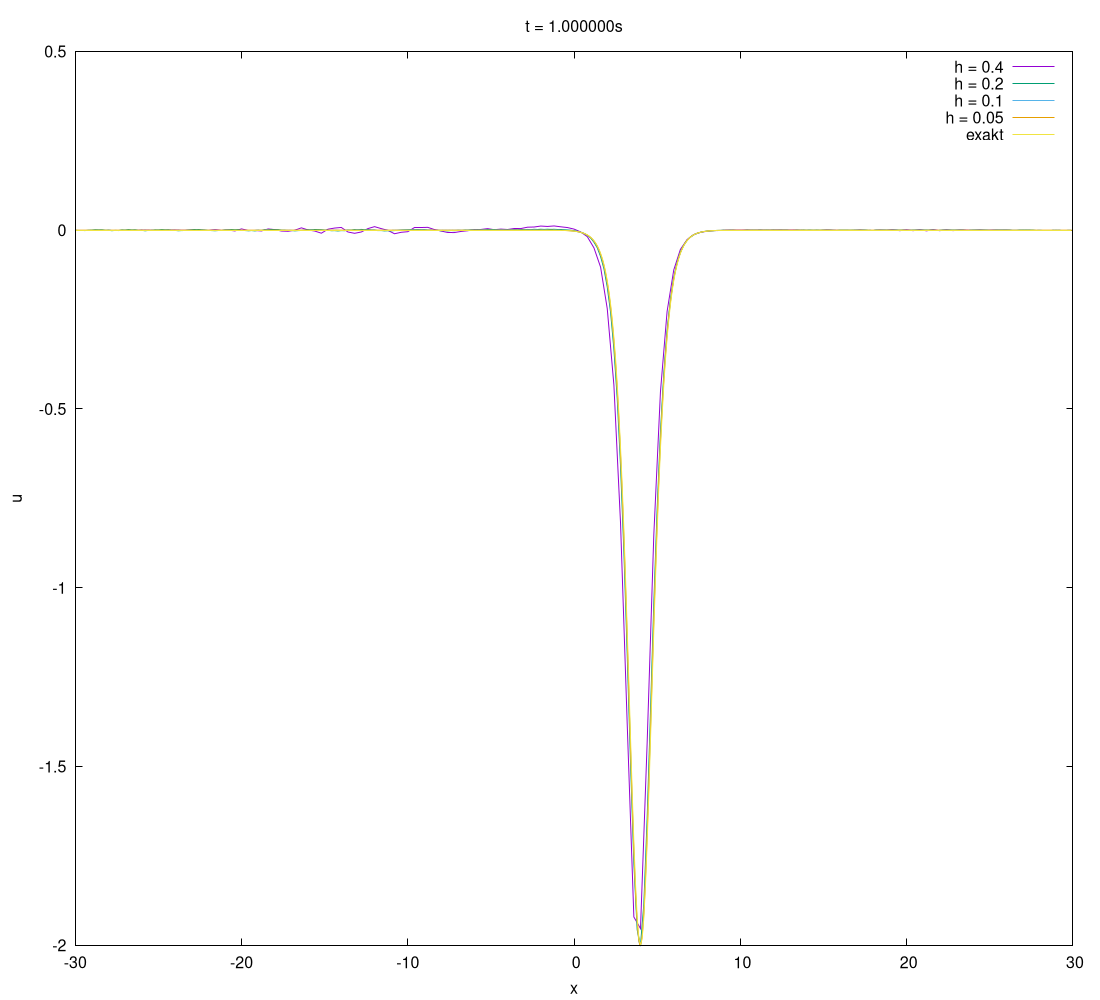
\includegraphics[width=0.88\textwidth]{vergleichN1.png}
	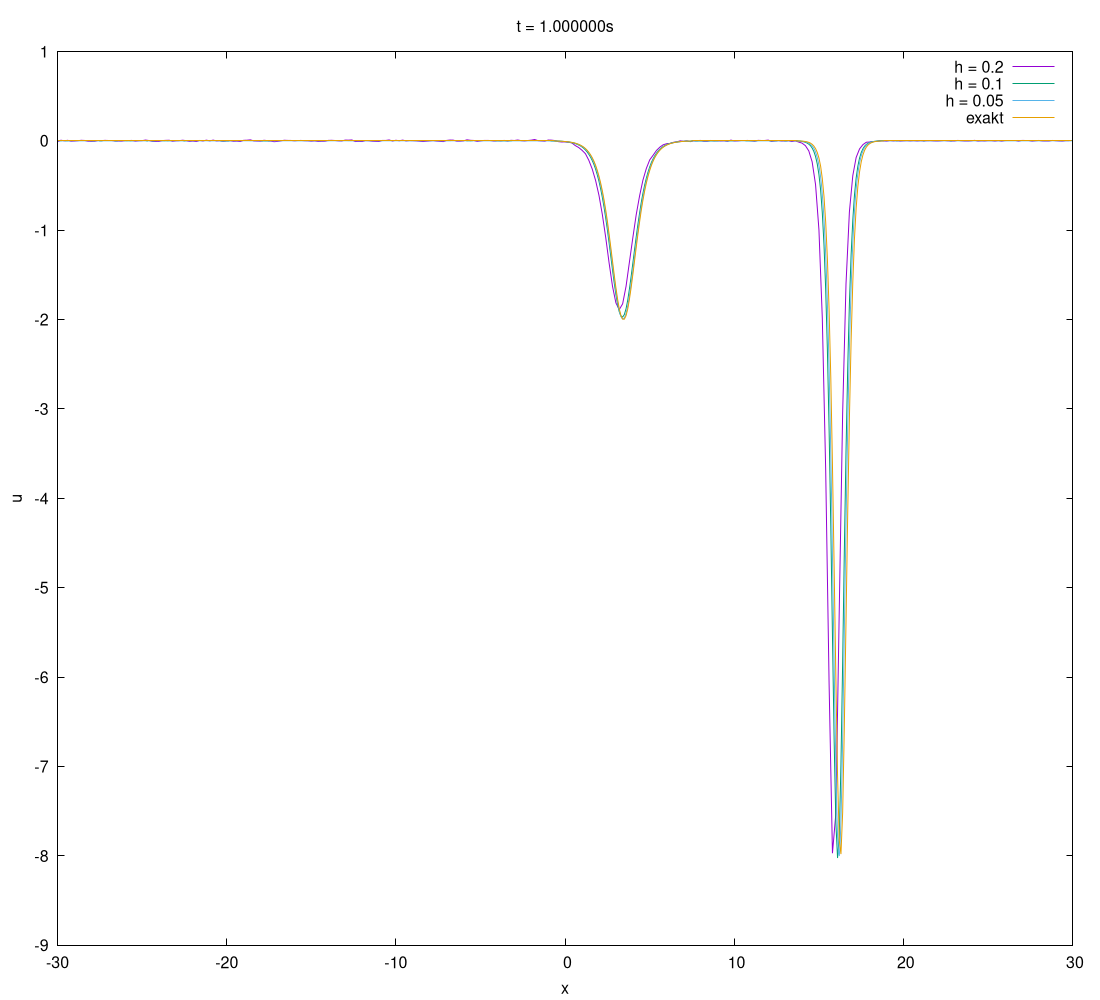
\includegraphics[width=0.88\textwidth]{vergleichN2.png}
	\caption[Vergleich]{Vergleich der numerischen und analytischen Lösung $u^{[1]}(1,x)$ (oben) und $u^{[2]}(1,x)$ (unten)}
	\label{fig:H10.22}
\end{figure}
Man sieht, dass diese Kurven recht gut konvergieren.
Nur $h=0.4$ konvergiert f\"ur $N=2$ nicht.
Um diese Konvergenz genauer zu untersuchen haben wir f\"ur alle
$d\in[3\cdot10^{-5},2.5\cdot10^{-4}]$
und alle $h\in[0.05,0.4]$
die Gesamtabweichung des numerischen Verfahren f\"ur $u^{[1]}$ und $u^{[2]}$
berechnet und in eine Heatmap geplottet.
Zusätzlich haben wir $d=\frac{1}{2.6}h^3$ geplottet, um zu zeigen, dass das
Verfahren f\"ur größere $d$ nicht konvergiert.
In Abbildung \ref{fig:H10.2} sieht man außerdem, dass $u^{[2]}$ eine 
viel st\"arkere h-Abh\"angigkeit hat als $u^{[1]}$, was man auch in der Abbildung \ref{fig:H10.22} gesehen hat.

\begin{figure}[htbp]
	\centering
	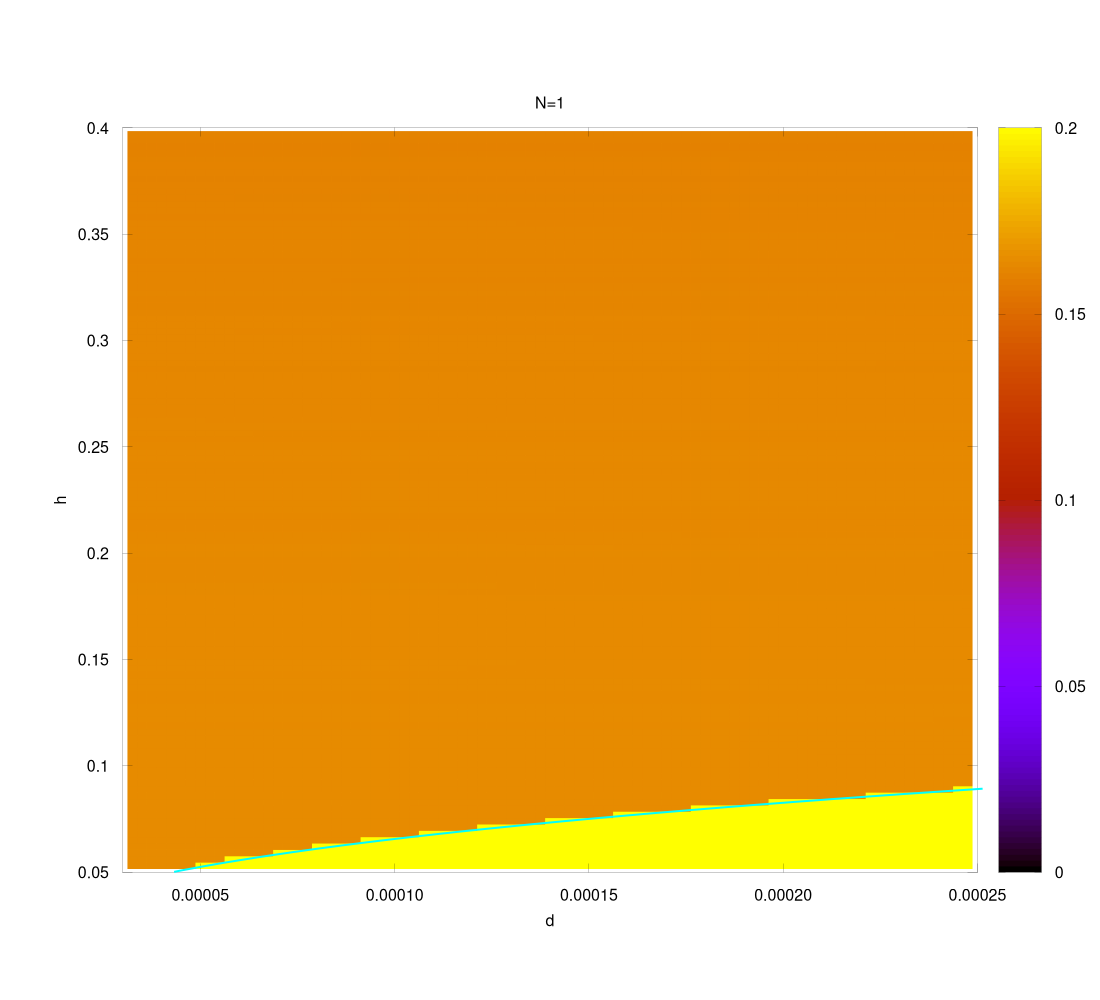
\includegraphics[width=0.9\textwidth]{heatMapN1}
	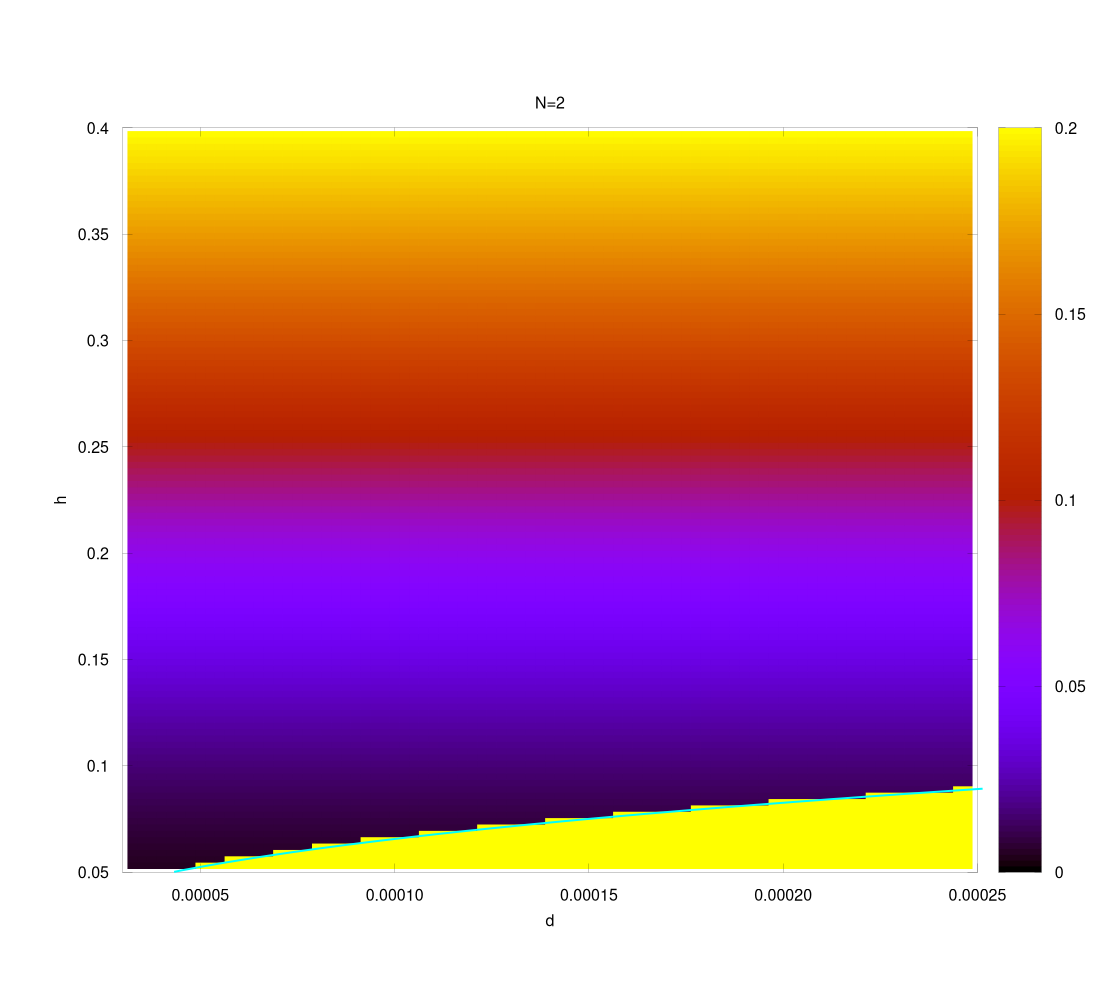
\includegraphics[width=0.9\textwidth]{heatMapN2}
	\caption[Vergleich]{Vergleich der Differenzen der numerischen und analytischen Lösung der DGL für $N=1$ (oben) und $N=2$ (unten)}
	\label{fig:H10.2}
\end{figure}
\subsection{}

Nun haben wir $u^{[3]}(t, x)$ numerisch in den Intervallen $t \in[0,1]$ und $x\in[-5,45]$ berechnet und im Video \ref{vid:H10.3} dargestellt. 
Man sieht drei Solitonen, die unterschiedliche Geschwindigkeiten und Amplituden haben.
Diese befinden sich alle bei $t=0$ am Ort $x=0$.

\begin{figure}[htbp]
	\centering
	\includemedia[
	width=0.5525\linewidth,height=0.5\linewidth,
	activate=pageopen,
	transparent,
	addresource=N3.mp4,
	flashvars={
		source=N3.mp4     % same path as in addresource!
		&loop=true           % loop video
		&scaleMode=letterbox % preserve aspect ratio
	}
	]{}{VPlayer9.swf}
	\caption[]{Hier ist $u^{[3]}(t, x)$ im Bereich von $t\in[0,1]$ und $t\in[-5,45]$ dargestellt.}
	\label{vid:H10.3}
\end{figure}
\subsection{}
Zuletzt betrachten wir Lösungen für $N\notin\mathbb{N}$.
Wir haben die Lösungen für $N\in[1.0,1.9]$ betrachtet und in Video \ref{vid:H10.4} dargestellt.
Man sieht, dass diese Anfangsbedingungen keine perfekten Solitonen ergeben;
Die resultierenden Kurven zerfließen leicht und erzeugen hinter sich Wellen, die auch positive Anteile haben.
Trotzdem erkennt man wie sich zwei immer besser getrennte Wellen bilden.

\begin{figure}[htbp]
	\centering
	\includemedia[
	width=0.5525\linewidth,height=0.5\linewidth,
	activate=pageopen,
	transparent,
	addresource=Nalle.mp4,
	flashvars={
		source=Nalle.mp4     % same path as in addresource!
		&loop=true           % loop video
		&scaleMode=letterbox % preserve aspect ratio
	}
	]{}{VPlayer9.swf}
	\caption[]{Hier ist $u^{[N]}(t, x)$ für $N\in[1.0,1.9]$ dargestellt.}
	\label{vid:H10.4}
\end{figure}
\end{document}


